
\section{Implementation}
\subsection{The Baseline}
\begin{figure}[!ht]
	\centering
	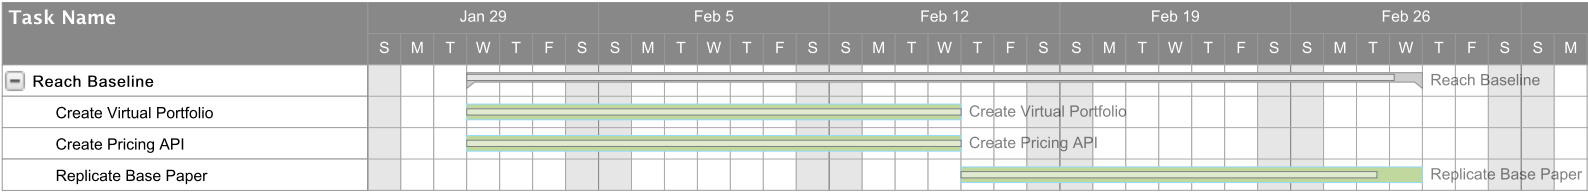
\includegraphics[width=\textwidth]{TWT_Gantt_1}
	\caption{Gantt Chart part 1}\label{fig:TWT_Gantt_1}
\end{figure}
The majority of the first section of the project has been completed.  Both the virtual portfolio and pricing API were created on schedule.  These were both necessary steps for the reproduction of the results in the baseline paper, “CrowdIQ: A New Opinion Aggregation Model”.  We are, however, behind schedule on the implementation of the baseline paper. 

Our stock price API retrieves and parses data from Yahoo Finance’s API, granting us access to several years worth of end-of-day financial data on a multitude of publicly traded companies.  The specific fields accessed are date, opening price, highest price, lowest price, closing price, and volume traded.  The getQuotes function takes a sequence of stock ticker symbols, a start date, and an end date as input, returning a map that contains end-of-day data for each trading day between the start and end dates.

The virtual portfolio allows us to fully simulate an investor’s stock market portfolio, allowing us to test trading strategies without investing real money.  The portfolio’s primary function is the management of three fields, the time, the money, and the stocks owned.  The portfolio does not run in real time, instead relying upon calls to a step function to progress the simulation by one trading day with each call.  The simulated money can be used in order to purchase stock, which is priced according the the previously mentioned stock pricing API.  The portfolio does not include commission fees or any other types of fees.

The combination of the stock price API and the virtual portfolio makes up our trading platform.  The TradingSimulation program makes a call to our stock price API requesting one year’s worth of data for ten different publicly traded companies, then stores this data into an HBase table.  It then initializes the virtual portfolio with \$100,000.  This portfolio is then controlled by a TradingStrategy, which utilizes both the tweet sentiment database and the recently-created stock-data database to make its decisions.

Using sentiment analysis combined with the API and portfolio described above we have been able to implement the trading algorithm present in the original paper. This is done by using a bank of tweets from 2014 provided to us and running them through a sentiment analysis provided by Saurabh and his partner Eric. Using this data the API and portfolio can make trades and measure them based on the real data from 2014 from the same time as the tweets. 

\subsection{Novel Trading Strategies}
\begin{figure}[!ht]
	\centering
	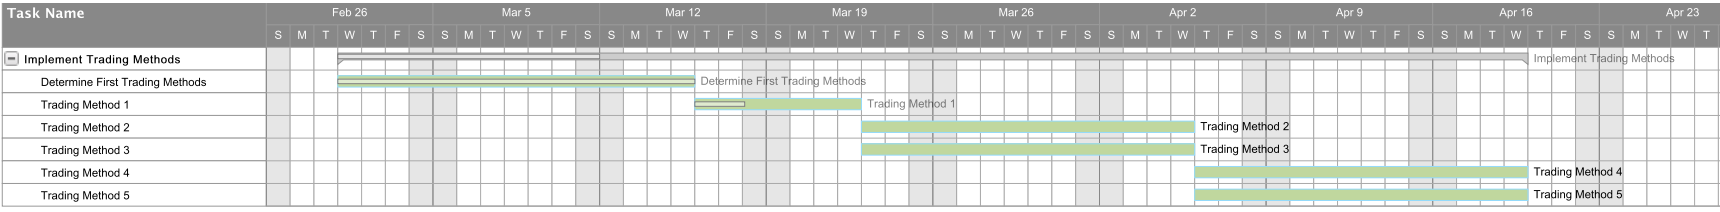
\includegraphics[width=\textwidth,keepaspectratio]{TWT_Gantt_2}
	\caption{Gantt Chart part 2}\label{fig:TWT_Gantt_2}
\end{figure}
As we finish up the implementation of the trading strategy that was reported in CrowdIQ, we have begun work on implementing our first novel trading strategy.  After completing this, we will split into two groups of two in order develop multiple new trading methods at once.  We should be able to work quickly on trading methods 2-5, allowing us to make up for the time that we had spent implementing the baseline algorithm.

While the exact trading strategies that we will be testing alongside the CrowdIQ paper are not fully set in stone we have a list of ideas that we would like to potentially test to see the results that occur. For example one of the trading strategies that the CrowdIQ paper doesn’t test is the idea of short selling stock and this is one of the first things we want to run tests with. The idea behind this is that not only would our program buy and sell stocks based upon the twitter sentiment that is derived, but it could also short sell stock given a set criteria. In fact this could then be taken further where we never sell stocks but only short sell stocks to see if that produces a significant difference. There are lots of possibilities of combinations and values that can be tweaked. While our current goal is 2-5 different additional strategies, we hope to do as many that we can.

In our current form of the code these different strategies are more or less hard written into the code as StockDecisions, StockActions, and StockOrchestrator classes. This is where the values for when to buy, when to sell, how much to buy, etc. are currently processed. As of right now these values are hard written into the code so that we can finish implementing the baseline paper. While this works for the current CrowdIQ implementation, it makes changing the calculation variables more complicated to modify. Since we will be adding more complexity to our trading strategies as this goes on, we plan to modify this slightly so that other techniques of trading will fit better into the code. While we do not need to run tests back to back or simultaneously, during the data analysis section of this project it would be useful to run several tests without much editing to the code in between. As this isn’t a current necessity this will be done if time permits.

One of the key features of this project is the twitter sentiment analysis. Since we have the 2014 sentiment analysis that the CrowdIQ paper used we plan to use that as our primary data set for all following trading strategies. Doing this will require no further implementation than what is already set up for the baseline test. As of this current moment we do not have any plans to test different forms of sentiment analysis. This will give us a constant to be able to compare all the following tests with. However, should time permit, changing the sentiment analysis would also be a good test to see how that would affect the success of the algorithm.

While the 2014 data set provides a large range of values to test with, it is still limited to a one year timespan. While we hypothesize that our results will not be significantly different from year to year, potential outliers are a possibility. To insure that we have a wider range of values we are also looking at using a web based technology called Quantopian.

Quantopian is a useful technology for this project because it allows you to implement code on their system to run on their data sets. This provides live feedback for how you implemented code performed. We hope that we will be able to use this as a method of testing our possible different strategies on different data sets. This will allow us to get more data so that we can further analyze which strategy will perform the most optimal. Quantopian works with Java so with minor changes to the code we should be able to quickly implement what we have written in Scala into Quantopian.


\subsection{Analysis and Presentation}
\begin{figure}[!ht]
	\centering
	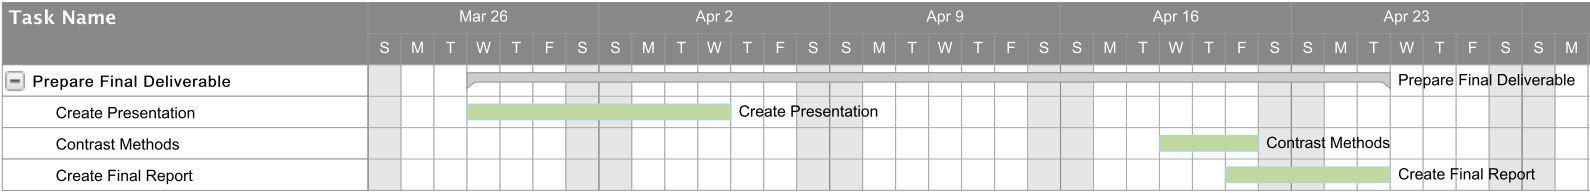
\includegraphics[width=\textwidth]{TWT_Gantt_3}
	\caption{Gantt Chart part 3}\label{fig:TWT_Gantt_3}
\end{figure}

After finishing development, our entire focus will be on comparing and contrasting the multiple trade strategies that we implemented in order to determine which algorithms were most effective and why they work so well.  While profit generated will certainly be a heavily weighted metric when determining which algorithm was most successful, it will certainly not be the only one.  Other metrics used for comparison will include risk, scalability, and volatility.

To determine the profit gained we will be comparing the profit gained to the overall stock market. This means that the profit each stock gained or lost over the year will be the baseline of comparison. We will then run our strategy and compare it to this baseline. As this runs, our virtual portfolio will be keeping track of our daily profit or loss. Whichever strategy ends up having the highest profit in the virtual portfolio at the end of the simulation will be the winner of this category.

Determining the risk of a given strategy is a lot more complicated than determining the profit. To determine this we will have to look at a couple different factors. The most critical factor to look at for the risk will be the number of mispredictions. For us a misprediction is considered when there is a buy but then the stock goes down without rebounding shortly after. A sell where the stock value continues to go up will also be considered a misprediction. Performing a short sell that doesn’t end up profitable will also count against the strategy. Upon comparing the number of mispredictions we will get a better idea as to what strategy is the “safest.” While a strategy might be very profitable, if it has a high risk, it might not be profitable on every data set. This is why we want to take this factor into consideration.

To figure out the scalability of the strategy we will be looking at using different number of purchases. While it is easy for the sentiment to tell us whether to buy or to sell, it can't give us a value for how much to sell. Because of this, different strategies will have different number of buys and sells. For example, when a buy action is determined, we can either use all our money and buy as much as we can, or we can buy 100 shares, 1 share, or \$1000 worth of stock. We will then expand how much initial funds we have in the portfolio and see how this scales. If a stock does very well starting with \$10,000 but does worse with perhaps \$100,000 then we will determine that this strategy does not scale well.

Determining the volatility of a given strategy will require use the techniques we used to determine both the risk and scalability. For us, a volatile strategy is one in which a misprediction causes a significant decrease in profit. Essentially a strategy in which there are significant spikes in income or loss becomes volatile. While significant increases are a good thing, we don’t want a profit pattern in which that increase drops shortly after. We want to be able to make an increase and hold that increase to get the optimal profit. This volatility can become more severe depending on how much we decided to buy or sell on each iteration. This is why it is important that we also consider the scalability when calculating this statistic. We will generally consider less volatile strategies to be more “optimal.”

Once we decide on the weights that we give to each category (profit, risk, scalability, volatility) we will then be able to see which trading strategy performs the best all around. However, this will also let others know which strategy is the best in certain categories so that a potential user can decide their own weights per category. Overall these four criteria will give us a very good understanding about how each strategy performs. All of this data will be collected and put into an excel spreadsheet as well as several different graphs. This will hopefully make the data as clear as possible to read.


%%% Local Variables:
%%% mode: latex
%%% TeX-master: "../report"
%%% End:
